%%%%%%%%%%%%%%%%%%%%%%%%%%%%%%%%%%%%%%%%%%%%%%%%%%%%%%%%%%%%%%%%%%%%%%%%%%%%%%%%
%%  Sample document for preparing papers to  "Avtomatika i Telemekhanika"
%%  charset=utf-8
%%%%%%%%%%%%%%%%%%%%%%%%%%%%%%%%%%%%%%%%%%%%%%%%%%%%%%%%%%%%%%%%%%%%%%%%%%%%%%%%

\documentclass[12pt]{a&t}
\usepackage{graphicx}
\usepackage{bm}
\usepackage{url}
\usepackage{multirow}

\usepackage{autonum}

\begin{document}  %%%!!!

\year{2020}
\title{Анализ моделей привилегированного обучения и дистилляции}%
\thanks{Работа выполнена при поддержке \dots
(грант \mbox{№\,\dots}).}

\authors{А.В.~ГРАБОВОЙ\\
(Московский физико-технический институт, Москва)\\
В.В.~СТРИЖОВ, д-р~физ-мат.~наук\\
(Вычислительный центр имени А.\,А. Дородницына ФИЦ ИУ РАН)}

\maketitle

\begin{abstract}
Данная работа посвящена методам понижения сложности аппроксимирующих моделей. Предлагается вероятностное обоснование методов дистилляции и привилегированного обучения. В работе приведены общие выводы для произвольной параметрической функции с наперед заданной структурой. Показано теоретическое обоснование для частных случаев: линейной и логистической регрессии. Проводится анализ рассмотренных моделей в вычислительном эксперименте на синтетических выборках и реальных данных. В качестве реальных данных рассматривается выборки FashionMNIST и Twitter Sentiment Analysis.

\smallskip\\
\textit{Ключевые слова}: выбор модели; байесовский вывод; дистилляция модели; привилегированное обучение.
\end{abstract}


\section{Введение}
Повышение точности аппроксимации в задачах машинного обучения влечет за собой повышение сложности моделей и как следствие снижает их интерпретируемость. Примером такого усложнения являются следующие модели: трансформеры~\cite{Vaswani2017}, BERT~\cite{Devlin2018}, ResNet~\cite{Kaiming2015} а также ансамбли этих моделей. 

При построении модели машинного обучения используется два свойства: сложность модели и точность аппроксимации модели. Сложность влияет на время, которое модель требуется для принятия решения, а также на интерпретируемость модели, следовательно модель которая имеют меньшую сложность является более предпочтительной~\cite{bachteev2018}. С другой стороны точность аппроксимации модели нужно максимизировать. В данной работе рассматривается метод \textit{дистилляции} модели. Данные метод позволяет строить новые модели на основе ранее обученых моделей.

\begin{definition}
Дистилляция модели~--- уменьшение сложности модели путем выбора модели в множестве более простых моделей с использованием ответов более сложной модели.
\end{definition}

В работе~\cite{Hinton2015} Дж.\,Е. Хинтоном рассматривается метод дистилляции моделей машинного обучения для задачи классификации. В работе проведен ряд экспериментов, в которых проводилась дистилляции моделей для разных задач машинного обучения. Эксперимент на выборке MNIST~\cite{mnist}, в котором избыточно сложно нейросеть была дистиллирована в нейросеть меньшей сложности. Эксперимент по Speech Recognition, в котором ансамбль моделей был \textit{дистиллирован} в одну модель. Также в работе~\cite{Hinton2015} был проведен эксперимент по обучению экспертных моделей на основе одной большой модели.

\begin{definition}
Привилегированная информация~--- множество признаков, которые доступны только в момент выбора модели, но не в момент тестирования.
\end{definition}

В работе~\cite{Vapnik2015} В.\,Н. Вапником введено понятия \textit{привилегированной информации}. В работе~\cite{Lopez2016} метод дистилляции~\cite{Hinton2015} используется вместе с привилегированным обучениям~\cite{Vapnik2015}. В предложенном методе на первом этапе обучается модель \textit{учителя} в пространстве привилегированной информации, после чего обучается модель \textit{ученика} в исходном признаковом пространстве используя \textit{дистилляцию}~\cite{Hinton2015}. Для обучения строится функция ошибки специального вида, анализируемая в данной работе. Эта функция состоит из нескольких слагаемых, включая ошибки учителя, ученика и регуляризирующие элементы.  Первые варианты подобной функции ошибки были предложены А.\,Г. Ивахненко~\cite{Ivakhnenko1994}.

\begin{definition}
Учитель~--- фиксируемая модель, ответы которой используются при выборе модели ученика.
\end{definition}

\begin{definition}
Ученик~--- модель, которая выбирается согласно какого-либо критерия.
\end{definition}

В данной работе предлагается рассмотреть вероятностный подход к решению задачи дистилляции модели и задачи привилегированного обучения. Подход обобщается на случай, когда привилегированная информация доступна не для всех объектов из обучающей выборки. В рамках вероятностного подхода предлагается анализ и обобщение функции ошибки~\cite{Hinton2015, Lopez2016}. Рассматриваются частные задачи классификации и регрессии~\cite{Ivakhnenko1994}.


В рамках вычислительного эксперимента анализируются методы использующие и не использующие модель учителя при обучение модели ученика. Для анализа используются реальные выборки для задачи классификации изображений FashionMNIST~\cite{fashionmnist} и для задачи классификации текстов Twitter Sentiment Analysis~\cite{twiter2013}. Выборка FashionMNIST использовалась вместо общепринятой выборки MNIST, так как последняя имеет приемлемое качество аппроксимации даже для линейного классификатора. Вычислительный эксперимент использует модели разной сложности: линейная модель, полносвязная нейронная сеть, сверточная нейронная сеть~\cite{LeCun1989}, модель Bi-LSTM~\cite{Schmidhuber1997} и модель BERT~\cite{Devlin2018}.

\section{Постановка задачи обучения с учителем}
Задано множество объектов~$\bm{\Omega}$ и множество целевых переменных~$\mathbb{Y}$. Множество~$\mathbb{Y}=\{1,\cdots,K\}$ для задачи классификации, где~$K$ число классов, множество $\mathbb{Y}=\mathbb{R}$ для задачи регрессии.
Для каждого объекта из~$\omega_i \in \bm{\Omega}$ задана целевая переменная~$\mathbf{y}_i = \mathbf{y}\bigr(\omega_i\bigr)$. Множество целевых переменных для всех объектов обозначим~$\mathbf{Y}$.
Для множества~$\bm{\Omega}$ задано отображение в некоторое признаковое пространство~$\mathbb{R}^{n}$:
\begin{gather}
\label{eq:st:phi}
\begin{aligned}
\varphi:\bm{\Omega} \to \mathbb{R}^{n}, \quad \left|\bm{\Omega}\right| = m,
\end{aligned}
\end{gather}
где~$n$ размерность признакового пространства, а~$m$ количество объектов в множестве~$\bm{\Omega}$. Отображение~$\varphi$ отображает объект~$\omega_i \in \bm{\Omega}$ в соответствующий ему вектор признаков $\mathbf{x}_i = \varphi(\omega_i)$.
Пусть для объектов~$\bm{\Omega}^* \subset \bm{\Omega}$ задана привилегированная информация:
\begin{gather}
\label{eq:st:phi*}
\begin{aligned}
\varphi^*:\bm{\Omega}^* \to \mathbb{R}^{n^*}, \quad \left|\bm{\Omega}^*\right| = m^*,
\end{aligned}
\end{gather}
где~$m^* \leq m$~--- число объектов с привилегированной информацией, $n^*$~--- число признаков в пространстве привилегированной информации. Отображение~$\varphi^*$ отображает объект~$\omega_i \in \bm{\Omega^*}$ в соответствующий ему вектор признаков $\mathbf{x}^*_i = \varphi^*(\omega_i)$.

Множество индексов объектов, для которых известна привилегированная информация, обозначим~$\mathcal{I}$:
\begin{gather}
\label{eq:st:3}
\begin{aligned}
\mathcal{I} = \{1 \leq i \leq m |~\text{для $i$-го объекта задана привилегированная информация}\},
\end{aligned}
\end{gather}
а множество индексов объектов, для которых не известна привилегированная информация, обозначим $\{1, \cdots, m\}\setminus \mathcal{I} = \bar{\mathcal{I}}$.

Пусть на множестве привилегированных признаков задана функция учителя~$\mathbf{f}\bigr(\mathbf{x}^*\bigr)$:
\begin{gather}
\label{eq:st:4}
\begin{aligned}
\mathbf{f}:\mathbb{R}^{n^*} \to \mathbb{Y}^*,
\end{aligned}
\end{gather}
где~$\mathbb{Y}^*=\mathbb{Y}$ для задачи регрессии и $\mathbb{Y}^*$ является единичным симплексом~$\mathcal{S}_K$ в пространстве размерности~$K$ для задачи классификации. Модель учителя~$\mathbf{f}$ ставит объекты~$\mathbf{X}^*$ в соответствие объектам~$\mathbf{S},$ то есть ~$\mathbf{f}\bigr(\mathbf{x}^*_i\bigr)=\mathbf{s}_i$.

Требуется выбрать модель ученика~$\mathbf{g}\bigr(\mathbf{x}\bigr)$ из множества:
\begin{gather}
\label{eq:st:G}
\begin{aligned}
\mathfrak{G} = \left\{\mathbf{g}| \mathbf{g}:\mathbb{R}^{n} \to \mathbb{Y}^*\right\},
\end{aligned}
\end{gather}
например для задачи классификации множество~$\mathfrak{G}$ может быть параметрическим семейством функций линейных моделей:
\begin{gather}
\label{eq:st:G:lin:cl}
\begin{aligned}
\mathfrak{G}_\text{lin,cl} = \left\{\mathbf{g}\bigr(\mathbf{W}, \mathbf{x}\bigr)| \mathbf{g}\bigr(\mathbf{W}, \mathbf{x}\bigr) = \textbf{softmax}\bigr(\mathbf{W}\mathbf{x}\bigr), \quad \mathbf{W} \in \mathbb{R}^{n\times K}\right\}.
\end{aligned}
\end{gather}

\section{Постановка задачи: Хинтона и Вапника}\label{state:hinton}
Рассмотрим описание метода предложеного в работах~\cite{Hinton2015, Lopez2016}. В рамках данных работ предполагается, что для всех данных доступна привилегированная информация~$\mathcal{I} = \{1, 2, \cdots, m\}$. В работе~\cite{Hinton2015} решается задача классификации вида:
\begin{gather}
    \mathfrak{D} = \{\left(\mathbf{x}_i, y_i\right)\}_{i=1}^{m}, \qquad \mathbf{x}_i \in \mathbb{R}^{n}, \quad y_i \in \mathbb{Y}=\{1, \cdots, K\},
\end{gather}
где~$y_i$~--- это класс объекта, также будем обозначать~$\mathbf{y}_i$ вектором вероятности для класса~$y_i$.

В постановке Хинтона рассматривается параметрическое семейство функций:
\begin{gather}
\label{eq:G:set:cl}
\mathfrak{G}_{\text{cl}} = \left\{\mathbf{g}| \mathbf{g} = \text{softmax}\bigr(\mathbf{z}\bigr(\mathbf{x}\bigr)/T\bigr), \quad \mathbf{z}: \mathbb{R}^n \to \mathbb{R}^K \right\},
\end{gather}
где~$\mathbf{z}$~--- это дифференцируемая параметрическая функция заданной структуры, $T$~--- параметр температуры. В качестве модели учителя~$\mathbf{f}$ рассматривается функция из множества~$\mathfrak{F}_{\text{cl}}$:
\begin{gather}
\label{eq:F:set:cl}
\mathfrak{F}_{\text{cl}} = \left\{\mathbf{f}| \mathbf{f} = \text{softmax}\bigr(\mathbf{v}\bigr(\mathbf{x}\bigr)/T\bigr), \quad \mathbf{v}: \mathbb{R}^n \to \mathbb{R}^K \right\},
\end{gather}
где~$\mathbf{v}$~--- это дифференцируемая параметрическая функция заданной структуры, $T$~--- параметр температуры.
Параметр температуры~$T$ имеет следующие свойства:
\begin{enumlist}
    \item при~$T\to 0$ получаем вектор, в котором один из классов имеет единичную вероятность;
    \item при~$T\to \infty$ получаем равновероятные классы.
\end{enumlist}

Функция потерь~$\mathcal{L}$ в которой учитывается перенос информации от модели учителя~$\mathbf{f}$ к модели ученика~$\mathbf{g}$ имеет следующий вид:
\begin{gather}
\label{eq:hinton:1}
\begin{aligned}
   \mathcal{L}_{st}\bigr(\mathbf{g}\bigr) = &-\sum_{i=1}^{m}\underbrace{{\sum_{k=1}^{K}y^k_i\log\mathbf{g}\bigr(\mathbf{x}_i\bigr)\bigr|_{T=1}}}_{\text{исходная функция потерь}}\\
   &-\sum_{i=1}^{m}\underbrace{{\sum_{k=1}^{K}\mathbf{f}\bigr(\mathbf{x}_i\bigr)\bigr|_{T=T_0}\log\mathbf{g}\bigr(\mathbf{x}_i\bigr)\bigr|_{T=T_0}}}_{\text{слагаемое дистилляция}},
\end{aligned}
\end{gather}
где~$\cdot\bigr|_{T=t}$ обозначает, что параметр температуры~$T$ в предыдущей функции равняется~$t$.

Получаем оптимизационную задачу:
\begin{gather}
\label{eq:hinton:opt}
\begin{aligned}
   \hat{\mathbf{g}} = \arg\min_{\mathbf{g} \in \mathfrak{G}_{\text{cl}}} \mathcal{L}_{st}\bigr(\mathbf{g}\bigr).
\end{aligned}
\end{gather}

Работа~\cite{Lopez2016} обобщает метод предложенный в работе~\cite{Hinton2015}. Решение задачи оптимизации~\eqref{eq:hinton:opt} зависит только от вектора ответов модели учителя~$\mathbf{f}$. Следовательно признаковые пространства учителя и ученика могут различаться. В этом случае получаем следующую постановку задачи:
\begin{gather}
    \mathcal{D} = \left\{\left(\mathbf{x}_i, \mathbf{x}^*_i, y_i\right)\right\}_{i=1}^{m}, \qquad \mathbf{x}_i \in \mathbb{R}^{n}, \quad \mathbf{x}^*_i \in \mathbb{R}^{n^*}, \quad y_i \in \{1, \cdots, K\},
\end{gather}
где~$\mathbf{x}_i$ это информация доступна на этапах обучения и контроля, а $\mathbf{x}^*_i$ это информация доступна только на этапе обучения. Модель учителя принадлежит множеству моделей~$\mathfrak{F}_{cl}^*$:
\begin{gather}
\label{eq:F:set:cl:priv}
\mathfrak{F}_{\text{cl}}^* = \left\{\mathbf{f}| \mathbf{f} = \text{softmax}\bigr(\mathbf{v}^*\bigr(\mathbf{x}^*\bigr)/T\bigr), \quad \mathbf{v}^*: \mathbb{R}^{n^*} \to \mathbb{R}^K \right\},
\end{gather}
где~$\mathbf{v}^*$~--- это дифференцируемая параметрическая функция заданной структуры, $T$~--- параметр температуры. Множество моделей~$\mathfrak{F}_{cl}^*$ отличается от множества моделей~$\mathfrak{F}_{cl}$ из выражения~\eqref{eq:F:set:cl}. В множестве~$\mathfrak{F}_{cl}$ модели используют пространство исходных признаков, а в множестве~$\mathfrak{F}_{cl}^*$ модели используют пространство привилегированных признаков. Функция потерь \eqref{eq:hinton:1} в случае модели учителя~$\mathbf{f} \in \mathfrak{F}_{cl}^*$ переписывается в следующем виде:
\begin{gather}
\label{eq:hinton:L:new}
\begin{aligned}
   \mathcal{L}_{st}\bigr(\mathbf{g}\bigr) = &-\sum_{i=1}^{m}{\sum_{k=1}^{K}y^k_i\log\mathbf{g}\bigr(\mathbf{x}_i\bigr)\bigr|_{T=1}}-\sum_{i=1}^{m}{\sum_{k=1}^{K}\mathbf{f}\bigr(\mathbf{x}^*_i\bigr)\bigr|_{T=T_0}\log\mathbf{g}\bigr(\mathbf{x}_i\bigr)\bigr|_{T=T_0}},
\end{aligned}
\end{gather}
где~$\cdot\bigr|_{T=t}$ обозначает, что параметр температуры~$T$ в предыдущей функции равняется~$t$.

Требуется построить модель, которая использует привилегированную информацию $\mathbf{x}^*_i$ при обучении. Для этого рассмотрим двухэтапную модель обучения предложенную в работе~\cite{Lopez2016}:
\begin{enumlist}
    \item выбираем оптимальную модель учителя $\mathbf{f} \in \mathfrak{F}_{\text{cl}}^*$;
    \item выбираем оптимальную модель ученика $\mathbf{g} \in \mathfrak{G}_{\text{cl}}$ используя дистилляцию~\cite{Hinton2015}. 
\end{enumlist}

Модель ученика~--- это функция, которая минимизирует \eqref{eq:hinton:L:new}. Модель учителя~--- это функция, которая минимизирует кросс--энтропийную функцию ошибки:
\begin{gather}
\label{eq:hinton.2}
\begin{aligned}
   \mathcal{L}_{th}\bigr(\mathbf{f}\bigr) = &-\sum_{i=1}^{m}{{\sum_{k=1}^{K}y^k_i\log\mathbf{f}\bigr(\mathbf{x}^*_i\bigr)}}.
   \end{aligned}
\end{gather}

\section{Постановка задачи: вероятностный подход}

\subsection{Метод максимального правдоподобия}
Задано распределения целевой переменной~$p\bigr(\mathbf{y}_i|\mathbf{x}_i, \mathbf{g}\bigr)$.
Для поиска~$\hat{\mathbf{g}}$ воспользуемся методом максимального правдоподобия. В качестве~$\hat{\mathbf{g}}$ выбирается функция, которая максимизирует правдоподобие модели:
\begin{gather}
\label{eq:st:7}
\begin{aligned}
\hat{\mathbf{g}} = \arg\max_{\mathbf{g}\in \mathfrak{G}} \prod_{i=1}^{N}p\bigr(\mathbf{y}_{i}|\mathbf{x}_i, \mathbf{g}\bigr),
\end{aligned}
\end{gather}
где множество~$\mathfrak{G}$ задается~\eqref{eq:st:G}.
\subsection{Подход дистилляции модели учителя в модель ученика}
Рассмотрим вероятностную постановку, в которой должны быть выполнены ограничения:
\begin{enumlist}
	\item задано распределение целевой переменной~$p\bigr(\mathbf{y}_i|\mathbf{x}_i, \mathbf{g}\bigr)$;
	\item задано совместное распределение целевой переменной и ответов модели учителя~$p\bigr(\mathbf{y}_i, \mathbf{s}_i|\mathbf{x}_i, \mathbf{g}\bigr)$;
	\item для всех $\omega \in \bm{\Omega}^*$ элементы $\mathbf{y}(\omega)$ и $\mathbf{s}(\omega)$ являются зависимыми величинами, так как ответы учителя должны коррелировать с истинными ответами;
	\item если $|\bm{\Omega}^*|=0$ то решение должно соответствовать решению~\eqref{eq:st:7}.
\end{enumlist}

Рассмотрим совместное правдоподобие истинных меток и меток учителя:
\begin{gather}
\label{eq:st:8}
\begin{aligned}
p\bigr(\mathbf{Y}, \mathbf{S}|\mathbf{X}, \mathbf{g}, \mathcal{I}\bigr)=\prod_{i\not\in \mathcal{I}}p\bigr(\mathbf{y}_i|\mathbf{x}_i, \mathbf{g}\bigr)\prod_{i\in \mathcal{I}}p\bigr(\mathbf{y}_i, \mathbf{s}_i|\mathbf{x}_i, \mathbf{g}\bigr).
\end{aligned}
\end{gather}
Расспишем~$p\bigr(\mathbf{y}_i, \mathbf{s}_i|\mathbf{x}_i, \mathbf{g}\bigr)$ по формуле условной вероятности:
\begin{gather}
\label{eq:st:bernuli}
\begin{aligned}
p\bigr(\mathbf{y}_i, \mathbf{s}_i|\mathbf{x}_i, \mathbf{g}\bigr) = p\bigr(\mathbf{y}_i|\mathbf{x}_i, \mathbf{g}\bigr)p\bigr(\mathbf{s}_i|\mathbf{y}_i, \mathbf{x}_i, \mathbf{g}\bigr)
\end{aligned}
\end{gather}
Подставляя выражения~\eqref{eq:st:bernuli} в~\eqref{eq:st:8} получаем.
\begin{gather}
\label{eq:st:9}
\begin{aligned}
p\bigr(\mathbf{Y}, \mathbf{S}|\mathbf{X}, \mathbf{g}, \mathcal{I}\bigr)=\prod_{i\not\in \mathcal{I}}p\bigr(\mathbf{y}_i|\mathbf{x}_i, \mathbf{g}\bigr)\prod_{i\in \mathcal{I}}p\bigr(\mathbf{y}_i|\mathbf{x}_i, \mathbf{g}\bigr)\prod_{i\in \mathcal{I}}p\bigr(\mathbf{s}_i|\mathbf{y}_i, \mathbf{x}_i, \mathbf{g}\bigr).
\end{aligned}
\end{gather}
Заметим, что~$\mathbf{y}_i$ и~$\mathbf{s}_i$ зависимы только через переменную~$\mathbf{x}_i$, тогда~$p\bigr(\mathbf{s}_i|\mathbf{y}_i, \mathbf{x}_i, \mathbf{g}\bigr)=p\bigr(\mathbf{s}_i|\mathbf{x}_i, \mathbf{g}\bigr)$. Получаем совместное правдоподобие:
\begin{gather}
\label{eq:st:10}
\begin{aligned}
p\bigr(\mathbf{Y}, \mathbf{S}|\mathbf{X}, \mathbf{g}, \mathcal{I}\bigr)=\prod_{i\not\in \mathcal{I}}p\bigr(\mathbf{y}_i|\mathbf{x}_i, \mathbf{g}\bigr)\prod_{i\in \mathcal{I}}p\bigr(\mathbf{y}_i|\mathbf{x}_i, \mathbf{g}\bigr)\prod_{i\in \mathcal{I}}p\bigr(\mathbf{s}_i|\mathbf{x}_i, \mathbf{g}\bigr).
\end{aligned}
\end{gather}
Используя~\eqref{eq:st:10} получаем следующую оптимизационную задачу для поиска~$\hat{\mathbf{g}}$
\begin{gather}
\label{eq:st:11}
\begin{aligned}
\hat{\mathbf{g}} = \arg\max_{\mathbf{g}\in \mathcal{G}} \prod_{i\not\in \mathcal{I}}p\bigr(\mathbf{y}_i|\mathbf{x}_i, \mathbf{g}\bigr)\prod_{i\in \mathcal{I}}p\bigr(\mathbf{y}_i|\mathbf{x}_i, \mathbf{g}\bigr)\prod_{i\in \mathcal{I}}p\bigr(\mathbf{s}_i|\mathbf{x}_i, \mathbf{g}\bigr).
\end{aligned}
\end{gather}
Для удобства, будем минимизировать логарифм, тогда из~\eqref{eq:st:11} получаем:
\begin{gather}
\label{eq:st:12}
\begin{aligned}
\hat{\mathbf{g}} = \arg\max_{\mathbf{g}\in \mathcal{G}} \sum_{i\not\in \mathcal{I}}\log p\bigr(\mathbf{y}_i|\mathbf{x}_i, \mathbf{g}\bigr) + \left(1-\lambda\right)\sum_{i\in \mathcal{I}}\log p\bigr(\mathbf{y}_i|\mathbf{x}_i, \mathbf{g}\bigr) + \lambda\sum_{i\in \mathcal{I}}\log p\bigr(\mathbf{s}_i|\mathbf{x}_i, \mathbf{g}\bigr),
\end{aligned}
\end{gather}
где параметр~$\lambda \in [0,1]$ введен для взвешивания ошибок на истинных ответах и ошибок относительно ответов учителя.

\begin{figure}[h!t]\center
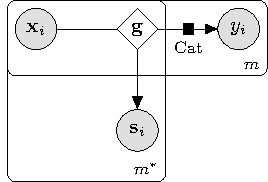
\includegraphics[width=0.35\textwidth]{figures/general_model}
\caption{Вероятностная модель в формате плоских нотаций.}
\label{fg:st:plate}
\end{figure}

На рис.~\ref{fg:st:plate} показан вид вероятностной модели в графовой нотации, для произвольной функции~$\mathbf{g}$. Для каждой реализации~$\mathbf{g}$ соответсвующий блок требует уточнение. На рис~\ref{fg:ex:synt:plate} показана более подробная реализация в случае, когда модель~$\mathbf{g}$ это линейная модель.

\section{Обучение с учителем для задачи классификации и регрессии}
\subsection{Случай классификации}
Для задачи многоклассовой классификации рассматриваются следующие вероятностные предположения:
\begin{enumlist}
\label{st:class:1}
	\item рассматривается функция учителя $\mathbf{f}\in\mathfrak{F}_{\text{cl}}^{*}$~\eqref{eq:F:set:cl:priv};
	\item рассматривается функция ученика следующего вида $\mathbf{g}\in\mathfrak{G}_{\text{cl}}$~\eqref{eq:G:set:cl};
	\item для истинных меток рассматривается категориальное распределение~$p\bigr(y|\mathbf{x}, \mathbf{g}\bigr) = \text{Cat}\bigr(\mathbf{g}\bigr(\mathbf{x}\bigr)\bigr)$, где $\mathbf{g}\bigr(\mathbf{x}\bigr)$ задает вероятность каждого класса;
	\item для меток учителя введем плотность распределения
\begin{gather}
\label{reg:dist}
\begin{aligned}
	p\bigr(\mathbf{s}|\mathbf{x}, \mathbf{g}\bigr) = C\prod_{k=1}^{K}g_k\bigr(\mathbf{x}\bigr)^{s^k},
\end{aligned}
\end{gather}
где~$g^k$ обозначает вероятность класса~$k$, которую предсказывает модель ученика, а~$s^k$~--- вероятность класса~$k$, которую предсказывает модель учителя.
\end{enumlist}
\begin{theorem}
\label{theorem:st:dist}
Пусть вероятнось каждого класса отделима от нуля и единицы, то есть для всех $k$ выполняется $1 > 1- \varepsilon > g_k\bigr(\mathbf{x}\bigr) > \varepsilon > 0,$ тогда при
\begin{gather}
C=\left(-1\right)^{K}\frac{K^{K/2}}{2^{K(K-1)/2}}\prod_{k=1}^{K}g_k\bigr(\mathbf{x}\bigr)\log g_k\bigr(\mathbf{x}\bigr)
\end{gather}
функция $p\bigr(\mathbf{s}|\mathbf{x}, \mathbf{g}\bigr)$ определенная в~\eqref{reg:dist} является плотностью распределения.
\end{theorem}
\begin{proof}
	Во-первых покажем, что для произвольного вектора ответов $\mathbf{s} \in \mathcal{S}_K$ выполняется $p\bigr(\mathbf{s}|\mathbf{x}, \mathbf{g}\bigr) \geq 0$. Заметим, что для всех~$k$ выполняется, что~$\log g_k\bigr(\mathbf{x}\bigr) < 0,$ тогда
\begin{gather}
\begin{aligned}
	C=\underbrace{\frac{K^{K/2}}{2^{K(K-1)/2}}}_{>0}\prod_{k=1}^{K}\underbrace{g_k\bigr(\mathbf{x}\bigr)}_{>\varepsilon}\underbrace{\left(-\log g_k\bigr(\mathbf{x}\bigr)\right)}_{>0} > 0,
\end{aligned}
\end{gather}
тогда с учетом того, что~$g_k\bigr(\mathbf{x}\bigr) >0$ и~$C>0$ получаем, что $p\bigr(\mathbf{s}|\mathbf{x}, \mathbf{g}\bigr) \geq 0$.
	Во-вторых покажем, что интеграл по всему пространству ответов~$\mathcal{S}_K$ является конечным:
	\begin{gather}
	\label{theorem:st:dist:eq:1}
	\begin{aligned}
		\int_{\mathcal{S}_K}p\bigr(\mathbf{s}|\mathbf{x}, \mathbf{g}\bigr)ds &= \int_{\mathcal{S}_K}\prod_{k=1}^{K}g_k\bigr(\mathbf{x}\bigr)^{s^k}ds = \prod_{k=1}^{K}\int_{\mathcal{S}_K}g_k\bigr(\mathbf{x}\bigr)^{s^k}ds\\ 
		& = \prod_{k=1}^{K}\int_{0}^{1}\frac{r^{K-1}\sqrt{K}}{\left(K-1\right)!\sqrt{2^{K-1}}}g_k\bigr(\mathbf{x}\bigr)^{r}dr = \prod_{k=1}^{K}\underbrace{\frac{\sqrt{K}}{\left(K-1\right)!\sqrt{2^{K-1}}}}_{D}\int_{0}^{1}r^{K-1}g_k\bigr(\mathbf{x}\bigr)^{r}dr \\
		& = D^K\prod_{k=1}^{K} \int_{0}^{1}r^{K-1}\exp\bigr(r\log g_k\bigr(\mathbf{x}\bigr)\bigr)dr \\
		& = \left(-D\right)^K\prod_{k=1}^{K}\log g_k\bigr(\mathbf{x}\bigr)\left(\Gamma\bigr(K\bigr) - \Gamma\bigr(K, -\log g_k\bigr(\mathbf{x}\bigr)\bigr)\right) \\
		& = \left(-D\right)^K\left(K-1\right)!^K\prod_{k=1}^{K}\log g_k\bigr(\mathbf{x}\bigr)\left(1 -g_k\bigr(\mathbf{x}\bigr) \exp_{K-1}\bigr(-\log g_k\bigr(\mathbf{x}\bigr)\bigr)+g_k\bigr(\mathbf{x}\bigr)\right) \\
		& = \frac{\left(-\sqrt{K}\right)^K}{2^{K(K-1)/2}}\prod_{k=1}^{K}\log g_k\bigr(\mathbf{x}\bigr)\left(1 -g_k\bigr(\mathbf{x}\bigr) \exp_{K-1}\bigr(-\log g_k\bigr(\mathbf{x}\bigr)\bigr)+g_k\bigr(\mathbf{x}\bigr)\right) < \infty,
	\end{aligned}
	\end{gather}
где~$\Gamma\bigr(K\bigr)$ является гамма функцией, $\Gamma\bigr(K, -\log g_k\bigr(\mathbf{x}\bigr)\bigr)$ является неполной гамма функцией, $\exp_{n}\bigr(x\bigr)$ является суммой Тейлора из первых~$n$ слагаемых. В рамках приближенных расчетов будем считать, что $\exp_{n}\bigr(x\bigr)\approx\exp\bigr(x\bigr),$ тогда с учетом~\eqref{theorem:st:dist:eq:1} получаем:
	\begin{gather}
	\label{theorem:st:dist:eq:2}
	\begin{aligned}
		C\bigr(\mathbf{g}, \mathbf{x}\bigr) = \int_{\mathcal{S}_K}p\bigr(\mathbf{s}|\mathbf{x}, \mathbf{g}\bigr)ds \approx \left(-1\right)^{K}\frac{K^{K/2}}{2^{K(K-1)/2}}\prod_{k=1}^{K}g_k\bigr(\mathbf{x}\bigr)\log g_k\bigr(\mathbf{x}\bigr)
	\end{aligned}
	\end{gather}
	
Полученное выражение~\eqref{theorem:st:dist:eq:2} заканчивает доказательство теоремы.
\end{proof}

Из теоремы~\ref{theorem:st:dist} следует, что плотность введенная для меток учителя является плотностью распределения, следовательно можно воспользоваться выражением~\eqref{eq:st:12}.
Используя предположения~1)--4) и подставляя в~\eqref{eq:st:12} получаем следующую оптимизационную задачу:
\begin{gather}
\label{eq:st:class:1}
\begin{aligned}
\hat{\mathbf{g}} = \arg\max_{\mathbf{g}\in \mathcal{G}} & \sum_{i\not\in \mathcal{I}}\sum_{k=1}^{K}y_i^k\log g_k\bigr(\mathbf{x}_i\bigr)\bigr|_{T=1} \\
&+ \left(1-\lambda\right)\sum_{i\in \mathcal{I}}\sum_{k=1}^{K}y_i^k\log g_k\bigr(\mathbf{x}_i\bigr)\bigr|_{T=1} + \lambda\sum_{i\in \mathcal{I}}\sum_{k=1}^{K}s_{i,k}\log g_k\bigr(\mathbf{x}_i\bigr)\bigr|_{T=T_0} \\
&+ \lambda \sum_{i\in \mathcal{I}}\sum_{k=1}^{K}\left(\log g_k\bigr(\mathbf{x}_i\bigr)\bigr|_{T=T_0} + \log\log\frac{1}{g_k\bigr(\mathbf{x}_i\bigr)}\bigr|_{T=T_0}\right),
\end{aligned}
\end{gather}
где выражение $\cdot\bigr|_{T=t}$ обозначает, что в предыдущую функцию $\text{softmax}$ требуется подставить значение температуры~$T$ равное некоторому значению~$t$.

Проанализировав выражение~\eqref{eq:st:class:1} получаем, что первые три слагаемые совпадают со слагаемыми в выражении~\eqref{eq:hinton:1} при~$\mathcal{I} = \{1, \cdots, m\},$ и $\lambda=\frac{1}{2}$, а четвертое слагаемое является некоторым регуляризатором, который получен из вида распределения.

Анализируя первые три слагаемых в выражении~\eqref{eq:st:class:1} получаем, что при~$T_0 = 1$ получаем сумму кросс энтропий между двумя распределениями для каждого объекта:
\begin{enumlist}
	\item первое распределение это выпуклая комбинация с весом~$1-\lambda$ и $\lambda$: распределения задаваемое метками объектов~$\text{Cat}\bigr(\mathbf{y}\bigr)$ и распределения задаваемого моделью учителя~$\text{Cat}\bigr(\mathbf{s}\bigr)$
	\item второе распределение это распределение задаваемое моделью ученика~$\text{Cat}\bigr(\mathbf{g}\bigr(\mathbf{x}\bigr)\bigr)$.
\end{enumlist}
Получаем, что модель ученика восстанавливает плотность не исходных меток, а новую плотность, которая является выпуклой комбинаций плотности исходных меток и меток учителя.
\subsection{Случай регрессии}
Для задачи регрессии рассматриваются следующие вероятностные предположения:
\begin{enumlist}
	\item рассматривается функция учителя~$\mathbf{f}\in\mathfrak{F}_{\text{rg}}^{*}$:
	\begin{gather}
	\label{eq:F:set:priv}
	\begin{aligned}
	\mathfrak{F}_{\text{rg}}^* = \left\{\mathbf{f}| \mathbf{f} = \mathbf{v}^*\bigr(\mathbf{x}^*\bigr), \quad \mathbf{v}^*: \mathbb{R}^{n^*} \to \mathbb{R} \right\},
	\end{aligned}
	\end{gather}
	где~$\mathbf{v}^*$~--- это дифференцируемая параметрическая функция;
	\item рассматривается функция ученика~$\mathbf{g}\in\mathfrak{G}_{\text{rg}}$:
\begin{gather}
\label{eq:G:set:rg}
\mathfrak{G}_{\text{rg}} = \left\{\mathbf{g}| \mathbf{g} = \mathbf{z}\bigr(\mathbf{x}\bigr), \quad \mathbf{z}: \mathbb{R}^n \to \mathbb{R}^K \right\},
\end{gather}
где~$\mathbf{z}$~--- это дифференцируемая параметрическая функция;
	\item истинные метки имеют нормальное распределение
	\begin{gather}
		p\bigr(y|\mathbf{x}, \mathbf{g}\bigr) = \mathcal{N}\bigr(y|\mathbf{g}\bigr(\mathbf{x}\bigr), \sigma\bigr);
	\end{gather}
	\item метки учителя распределены
	\begin{gather}
		p\bigr(s| \mathbf{x}, \mathbf{g}\bigr) = \mathcal{N}\bigr(s|\mathbf{g}\bigr(\mathbf{x}\bigr), \sigma_s\bigr);
	\end{gather}
\end{enumlist}

Используя предположения~1)--4) и подставляя в~\eqref{eq:st:12} получаем следующую оптимизационную задачу:
\begin{gather}
\label{eq:st:reg:1}
\begin{aligned}
\hat{g} = \arg\min_{g\in \mathcal{G}} & \sum_{i\not\in \mathcal{I}}\sigma^2\left(y_i-\mathbf{g}\bigr(\mathbf{x}_i\bigr)\right)^2 \\
&+ \left(1-\lambda\right)\sum_{i\in \mathcal{I}}\sigma^2\left(y_i-\mathbf{g}\bigr(\mathbf{x}_i\bigr)\right)^2 + \lambda\sum_{i\in \mathcal{I}}\sigma_s^2\left(s_i-\mathbf{g}\bigr(\mathbf{x}_i\bigr)\right)^2.
\end{aligned}
\end{gather}
Выражение~\eqref{eq:st:reg:1} записано с точностью до аддитивной константы относительно~$\mathbf{g}$. 

\begin{theorem}
\label{theorem:st:reg}
Пусть множество~$\mathcal{G}$ описывает класс линейных функций вида~$\mathbf{g}\bigr(\mathbf{x}\bigr) = \mathbf{w}^{\mathsf{T}}\mathbf{x}.$ Тогда решение оптимизационной задачи~\eqref{eq:st:reg:1} эквивалентно решению следующей задачи линейной регрессии:
\begin{gather}
\label{eq:st:reg:th:st:1}
\begin{aligned}
\mathbf{y''} = \mathbf{X}\mathbf{w} + \bm{\varepsilon},~\bm{\varepsilon} \sim \mathcal{N}\bigr(\mathbf{0}, \bm{\Sigma}\bigr),
\end{aligned}
\end{gather}
где $\bm{\Sigma}^{-1}=\text{diag}\bigr(\bm{\sigma'}\bigr)$ и $\mathbf{y''}$ имеют следующий вид:
\begin{gather}
\label{eq:st:reg:th:st:2}
\begin{aligned}
\sigma'_{i} &= \begin{cases}
\sigma^2,~\text{если}~i \not \in \mathcal{I}\\
\left(1-\lambda\right)\sigma^2+\lambda\sigma_s^2,~\text{иначе}\\
\end{cases}, \\
\mathbf{y''} &= \bm{\Sigma}\mathbf{y'},\\
y'_i &= \begin{cases}
\sigma^2y_i,~\text{если}~i \not \in \mathcal{I}\\
\left(1-\lambda\right)\sigma^2y_i+\lambda\sigma_s^2s_i,~\text{иначе}\\
\end{cases}.
\end{aligned}
\end{gather}
\end{theorem}
\begin{proof}
Обозначеним~$\mathbf{a}_{\mathcal{J}} = [a_i| i \in \mathcal{J}]^{\mathsf{T}},$ где~$\mathbf{a}$ произвольный вектор, а $\mathcal{J}$ произвольное не пустое индексное множество. Подвектор вектора ответов~$\mathbf{y}$, для элементов которого доступна привилегированная информация обозначим $\mathbf{y}_{\mathcal{I}} = [y_i| i \in \mathcal{I}]^{\mathsf{T}}$. Аналогично обозначим матрицу~$\mathbf{X}_\mathcal{I}=[\mathbf{x}_{i}| i \in \mathcal{I}]^{\mathsf{T}}$.

В случае линейной модели~$\mathbf{g}\bigr(\mathbf{x}\bigr) = \mathbf{w}^{\mathsf{T}}\mathbf{x}$ выражение \eqref{eq:st:reg:1} принимает вид:
\begin{gather}
\label{eq:st:reg:2}
\begin{aligned}
\hat{\mathbf{w}} = \arg\min_{\mathbf{w}\in \mathcal{W}} &~ \sigma^2\left(\mathbf{y}_{\bar{\mathcal{I}}}-\mathbf{X}_{\bar{\mathcal{I}}}\mathbf{w}\right)^{\mathsf{T}}\left(\mathbf{y}_{\bar{\mathcal{I}}}-\mathbf{X}_{\bar{\mathcal{I}}}\mathbf{w}\right) \\
&+ \sigma^2\left(1-\lambda\right)\left(\mathbf{y}_{\mathcal{I}}-\mathbf{X}_{\mathcal{I}}\mathbf{w}\right)^{\mathsf{T}}\left(\mathbf{y}_{\mathcal{I}}-\mathbf{X}_{\mathcal{I}}\mathbf{w}\right) + \sigma^2_s\lambda\left(\mathbf{s}_{\mathcal{I}}-\mathbf{X}_{\mathcal{I}}\mathbf{w}\right)^{\mathsf{T}}\left(\mathbf{s}_{\mathcal{I}}-\mathbf{X}_{\mathcal{I}}\mathbf{w}\right).
\end{aligned}
\end{gather}

Раскроем скобки и сгруппируем:
\begin{gather}
\label{eq:st:reg:3}
\begin{aligned}
\hat{\mathbf{w}} = \arg\min_{\mathbf{w}\in \mathcal{W}} &~ \sigma^2\left(\mathbf{w}^{\mathsf{T}}\mathbf{X}^{\mathsf{T}}_{\bar{\mathcal{I}}}\mathbf{X}_{\bar{\mathcal{I}}}\mathbf{w} - 2\mathbf{y}^{\mathsf{T}}_{\bar{\mathcal{I}}}\mathbf{X}_{\bar{\mathcal{I}}}\mathbf{w}\right) \\
&+ \left(1-\lambda\right)\sigma^2\left(\mathbf{w}^{\mathsf{T}}\mathbf{X}^{\mathsf{T}}_{\mathcal{I}}\mathbf{X}_{\mathcal{I}}\mathbf{w}- 2\mathbf{y}^{\mathsf{T}}_{\mathcal{I}}\mathbf{X}_{\mathcal{I}}\mathbf{w}\right) + \lambda\sigma^2_s\left(\mathbf{w}^{\mathsf{T}}\mathbf{X}^{\mathsf{T}}_{\mathcal{I}}\mathbf{X}_{\mathcal{I}}\mathbf{w}- 2\mathbf{s}^{\mathsf{T}}_{\mathcal{I}}\mathbf{X}_{\mathcal{I}}\mathbf{w}\right)
\end{aligned}
\end{gather}
Продифференцируем выражение, приравняем к нулю и сгруппируем элементы:
\begin{gather}
\label{eq:st:reg:4}
\begin{aligned}
\left(\sigma^{2}\mathbf{X}^{\mathsf{T}}_{\bar{\mathcal{I}}}\mathbf{X}_{\bar{\mathcal{I}}} + \left(1-\lambda\right)\sigma^2\mathbf{X}^{\mathsf{T}}_{\mathcal{I}}\mathbf{X}_{\mathcal{I}} + \lambda\sigma^{2}_s\mathbf{X}^{\mathsf{T}}_{\mathcal{I}}\mathbf{X}_{\mathcal{I}}\right) \mathbf{w} =& 2\sigma^2\mathbf{X}^{\mathsf{T}}_{\bar{\mathcal{I}}}\mathbf{y}_{\bar{\mathcal{I}}} \\
&+ 2\left(1-\lambda\right)\sigma^2\mathbf{X}^{\mathsf{T}}_{\mathcal{I}}\mathbf{y}_{\mathcal{I}} + 2\lambda\sigma_s^2\mathbf{X}^{\mathsf{T}}_{\mathcal{I}}\mathbf{s}_{\mathcal{I}}.
\end{aligned}
\end{gather}
Воспользуемся следующими равенствами:
\begin{gather}
\label{eq:st:reg:simp}
\begin{aligned}
\sigma^{2}\mathbf{X}^{\mathsf{T}}_{\bar{\mathcal{I}}}\mathbf{X}_{\bar{\mathcal{I}}} + \left(1-\lambda\right)\sigma^2\mathbf{X}^{\mathsf{T}}_{\mathcal{I}}\mathbf{X}_{\mathcal{I}} + \lambda\sigma^{2}_s\mathbf{X}^{\mathsf{T}}_{\mathcal{I}}\mathbf{X}_{\mathcal{I}} &= \mathbf{X}^{\mathsf{T}}\bm{\Sigma}^{-1}\mathbf{X},\\
2\sigma^2\mathbf{X}^{\mathsf{T}}_{\bar{\mathcal{I}}}\mathbf{y}_{\bar{\mathcal{I}}} + 2\left(1-\lambda\right)\sigma^2\mathbf{X}^{\mathsf{T}}_{\mathcal{I}}\mathbf{y}_{\mathcal{I}} + 2\lambda\sigma_s^2\mathbf{X}^{\mathsf{T}}_{\mathcal{I}}\mathbf{s}_{\mathcal{I}} &= 2\mathbf{X}\mathbf{y'},
\end{aligned}
\end{gather}
где~$\bm{\Sigma}$ и~$\mathbf{y'}$ из условия задачи~\eqref{eq:st:reg:th:st:2}.

Подставляя~\eqref{eq:st:reg:simp} в~\eqref{eq:st:reg:4} получаем:
\begin{gather}
\label{eq:st:reg:5}
\begin{aligned}
\mathbf{w} = 2\left(\mathbf{X}^{\mathsf{T}}\bm{\Sigma}^{-1}\mathbf{X}\right)^{-1}\mathbf{X}\bm{\Sigma}^{-1}\mathbf{y''},
\end{aligned}
\end{gather}
что соответсвует решению задачи~\eqref{eq:st:reg:th:st:1}.
\end{proof}

Теорема~\ref{theorem:st:reg} показывает, что обучения с учителем для задачи регрессии можно свести к классической задаче оптимизации для задачи линейной регрессии.

\section{Вычислительный эксперимент}
Проводится вычислительный эксперимент для анализа качества моделей, которые получены путем дистилляции модели учителя в модель ученика. Как показано в теореме~\ref{theorem:st:reg} задачу регрессии с учителем можно свести к задаче регрессии без учителя, поэтому в эксперименте рассматривается только случай классификации. Во всех частях вычислительного эксперимента для поиска оптимальных параметров нейросетей использовался градиентный метод оптимизации ``Adam''~\cite{kingma2014}.
\subsection{Выборка FashionMNIST}
В данной части проводится эксперимент для задачи классификации для выборки FashionMNIST~\cite{fashionmnist}. В качестве модели учителя~$\mathbf{f}$ рассматривается модель нейросети с двумя сверточными слоями и с тремя полносвязными слоями, в качестве функции активации рассматривается ReLu. Модель учителя содержит~$~30$ тысяч обучаемых параметров. В качестве модели ученика рассматривается модель логистической регрессии для многоклассовой классификации. Модель ученика содержит~$7850$ обучаемых параметров.

\begin{figure}[h!t]\center
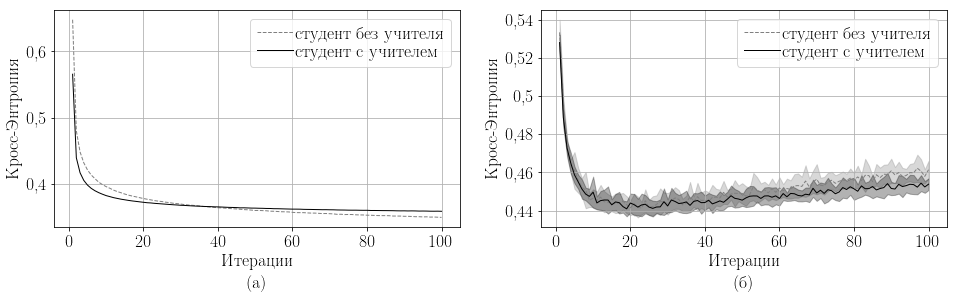
\includegraphics[width=1\textwidth]{figures/mnist_loss}
\caption{Зависимость кросс--этропии между истинными метками и предсказанными учеников вероятностями классов: a) на обучающей выборке; b) на тестовой выборке.}
\label{fg:ex:fashionmnist:loss}
\end{figure}

На рис.~\ref{fg:ex:fashionmnist:loss} показан график зависимости кросс--энтропии между истинными метками объектов и вероятностями, которые предсказывает модель ученика. На графике сравнивается моделя, которая обучалась без учителя (в задаче оптимизации~\eqref{eq:st:class:1} присутствует только первое слагаемое) с моделью, которая была получена путем дистилляции модели нейросети в линейную модель. На графике видно, что обе модели начинают переобучатся после 30-й итерации, но модель, которая получена путем дистилляции переобувается не так быстро, что следует из того, что ошибка на тестовой выборке растет медленней, а на обучающей выборке падает также медленней.


\subsection{Синтетический эксперимент}
Проанализируем модель на синтетической выборке. Выборка построенная следующим образом:
\begin{gather}
\begin{aligned}
\mathbf{W} &= \left[\mathcal{N}\bigr(w_{jk}|0, 1\bigr)\right]_{n\times K}, \quad &\mathbf{X} &= \left[\mathcal{N}\bigr(x_{ij}|0, 1\bigr)\right]_{m\times n}, \\
 \mathbf{S} &= \text{softmax}\left(\mathbf{XW}\right), \quad &\mathbf{y} &= \left[\text{Cat}\bigr(y_i| \mathbf{s}_i\bigr)\right],
\end{aligned}
\end{gather}
где функция~$\text{softmax}$ берется построчно. Строки матрицы~$\mathbf{S}$ будем рассматривать как предсказание учителя, то есть учитель знает истинные вероятности каждого класса. На рис.~\ref{fg:ex:synt:plate} показана вероятностная модель в графовой нотации. В эксперименте число признаков~$n=10$, число классов~$K=3$, для обучения было сгенерировано~$m_{\text{train}}=1000$ и~$m_{\text{test}}=100$ объектов.

На рис.~\ref{fg:ex:synt:distr:real} показано распределение по классам для~$20$ объектов из обучающей выборки. Каждому столбцу на графике соответствует объект, а каждой строке соответствует вероятность класс. Видно, что для каждого рассмотренного объекта вероятности разных классов близки. Получается, что если в качестве истинных меток взять класс с максимальной вероятностью, то выборка будет сильно зашумленной и модель будет описывать эти данные не корректно.

Построим в качестве ученика простую линейную модель, которая минимизирует крос--энтропийную (первое слагаемое в формуле~\eqref{eq:st:class:1}). Представление данной модели в виде графовой модели показано на рис.~\ref{fg:ex:synt:plate}.

\begin{figure}[h!t]\center
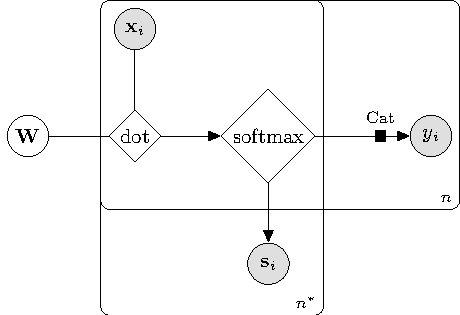
\includegraphics[width=0.35\textwidth]{figures/linear_model}
\caption{Вероятностная модель используемая в синтетическом эксперименте.}
\label{fg:ex:synt:plate}
\end{figure}

\begin{figure}[h!t]\center
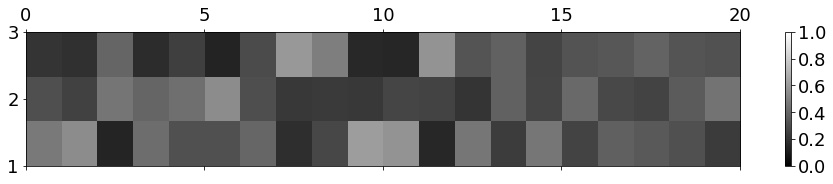
\includegraphics[width=1\textwidth]{figures/syn_real_distr}
\caption{Истинное распределение  объектов по классам.}
\label{fg:ex:synt:distr:real}
\end{figure}


На рис.~\ref{fg:ex:synt:distr:without} показано распределение вероятностей классов, которое предсказала модель. Видно, что полученное распределение не соответствует истинному, так как модель сосредотачивает всю вероятность в одном классе.

\begin{figure}[h!t]\center
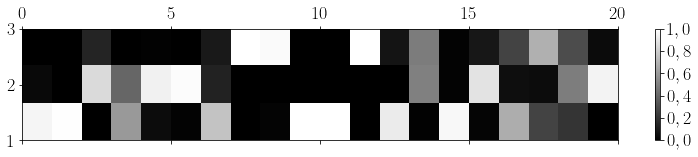
\includegraphics[width=1\textwidth]{figures/syn_without_teacher_distr}
\caption{Распределение предсказанное моделью без использования информации об истинном распределение на классах.}
\label{fg:ex:synt:distr:without}
\end{figure}

\begin{figure}[h!t]\center
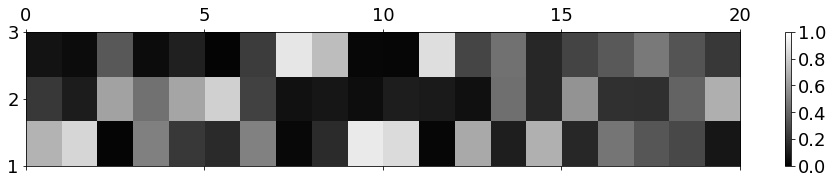
\includegraphics[width=1\textwidth]{figures/syn_with_teacher_distr}
\caption{Распределение предсказанное моделью используя информацию об истинном распределение на классах.}
\label{fg:ex:synt:distr:with}
\end{figure}

\begin{figure}[h!t]\center
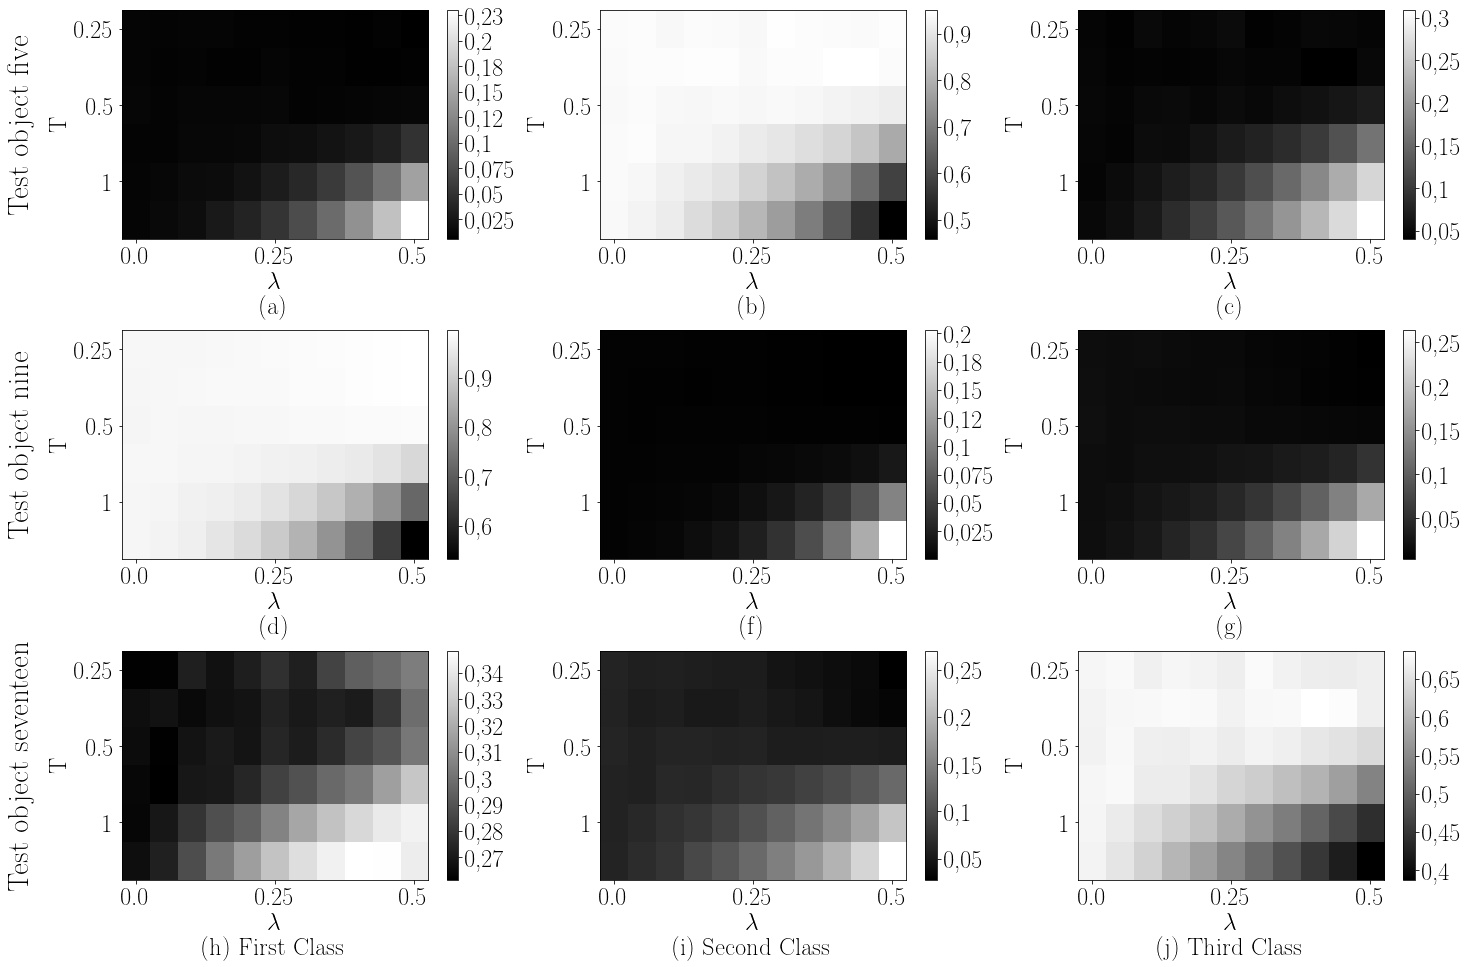
\includegraphics[width=1\textwidth]{figures/syn_T_lambda}
\caption{Иллюстрация распределения вероятности предсказания классов при различных значениях~$\lambda$ и $T$.}
\label{fg:ex:synt:distr:lambda_T}
\end{figure}

Рассмотрим модель, которая учитывает информацию об истинных распределениях на классах для каждого объекта. Для этого будем минимизировать первые три слагаемых в формуле~\eqref{eq:st:class:1}, при~$T_0=1$ и~$\lambda=0{,}75$. В качестве меток учителя~$s_{i,k}$ использовались истинные вероятности для каждого класса для данного объекта. На рис~\ref{fg:ex:synt:distr:with} показано распределение, которое дала модель в данном случае, видно, что распределения являются сглаженными и концентрации всей вероятности в одном классе не наблюдается.

Заметим, что в данном примере предполагается, что модель учителя учитывает не только метки классов, а и распределение на метках классов, в то время как в выборке~$\mathcal{D} = \{\mathbf{X}, \mathbf{y}\},$ имеются только точечные оценки в виде меткок. 

В данном примере используются истинные распределения в качестве предсказаний учителя, но их можно заменить предсказаниями модели учителя, которая предсказывает не только сами меток, а и их распределение для каждого объекта.

На рис.~\ref{fg:ex:synt:distr:lambda_T} показана зависимость вероятности верного класса от температуры~$T$ и параметра доверия~$\lambda$ для одного из объекта из тестовой выборке. На рисунке видно, что изменение температуры~$T$ влечет изменение концентрации вероятностной меры. При уменьшении параметра температуры к нулю, получаем, что вероятность одного из классов становиться близко к единице, а остальных близко к нулю. С другой стороны при увеличения параметра температуры вероятности классов сглаживаются и распределение классов для каждого объекта становится близким к равномерному.

В таблице~\ref{tb:ce:1} в колонке ``Кросс-Энтропийная ошибка с реальными вероятностями'' показано сравнение кросс--этропии в случае, если в качестве истинных вероятностей меток рассмотреть не onehot вероятности классов, а истинные вероятности. Видно, что модель с учителем лучше аппроксимирует истинные вероятности классов. Также в таблице~\ref{tb:ce:1} предсталенно среднее значение разницы максимальной вероятности с минимальной вероятностью для каждого объекта. Видно, что модель учителя имеет меньшую разнице между вероятностями классов, то есть вероятности классов не конценрируются в одном классе.

\subsection{Выборка Twitter Sentiment Analysis}
В данной части проводится эксперимент на выборке Twitter Sentiment Analysis. Данная выборка содержит короткие сообщения, для которых нужно предсказать эмоциональный окрас: содержит твит позитивный окрас или негативный. Выборка разделена на~$1{,}18$ миллиона твитов для обучения и~$0{,}35$ миллиона твитов для тестирования. В твитах была выполнена следующая предобработка:
\begin{itemize}
	\item все твиты были переведены в нижний регистр;
	\item все никнеймы вида~``@andrey'' были заменены на токен ``name'';
	\item все цифры были заменены на токен ``number''.
\end{itemize}
Результаты данной части эксперимента показаны в табл.~\ref{tb:ce:1}. В качестве модели учителя использовалась модель Bi-LSTM с~$170$ тысячами параметров для обучения. В качестве эмбедингов обучалась матрица из~$30$ миллионов параметров в единой процедуре с моделью BI-LSTM. Обученная модель учителя имеет точность предсказания~$0{,}835$. В качестве модели ученика рассматривается модель с $1538$ параметрами, но в качестве эмбедингов рассматривается переобученная модель BERT. В таблице~\ref{tb:ce:1} показано качество модели ученика используя предсказания модели учителя и без них.

Программное обеспечение для проведения экспериментов и проверки результатов находится в~\cite{Code2020}.

\section{Заключение}
\begin{table}[]
\caption{Сводная таблица результатов вычислительного эксперимента.}
\label{tb:ce:1}
\begin{center}
\resizebox{\textwidth}{!}{
\begin{tabular}{|l|c|c|c|c|c|c|}
\hline
\multicolumn{1}{|c|}{Выборка} & Модель      & \begin{tabular}[c]{@{}c@{}}Кросс-Энтропийная\\ ошибка\end{tabular} & \begin{tabular}[c]{@{}c@{}}Кросс-Энтропийная \\ ошибка с реальными\\ вероятностями\end{tabular} & \begin{tabular}[c]{@{}c@{}}Вероятностная\\ разница\end{tabular} & Точность            & \begin{tabular}[c]{@{}c@{}}Число\\ Параметров\end{tabular} \\ \hline
\multirow{2}{*}{FashionMnist} & с учителем  & $0{,}461\pm0{,}005$                                                & -                                                                                             & $0{,}84\pm0{,}13$                                               & $0{,}842\pm0{,}002$ & 7850                                                       \\ \cline{2-7} 
                              & без учителя & $0{,}453\pm0{,}003$                                                & -                                                                                             & $0{,}86\pm0{,}18$                                               & $0{,}841\pm0{,}002$ & 7850                                                       \\ \hline
\multirow{2}{*}{Systetic}     & с учителем  & $0{,}225\pm0{,}002$                                                & $1{,}17\pm0{,}05$                                                                             & $0{,}45\pm0{,}20$                                               & $0{,}831\pm0{,}002$ & 33                                                         \\ \cline{2-7} 
                              & без учителя & $0{,}452\pm0{,}001$                                                & $2{,}64\pm0{,}02$                                                                             & $0{,}75\pm0{,}22$                                               & $0{,}828\pm0{,}001$ & 33                                                         \\ \hline
\multirow{2}{*}{Twiter}       & с учителем  & $0{,}501\pm0{,}006$                                                & -                                                                                             & $0{,}79\pm0{,}17$                                               & $0{,}764\pm0{,}005$ & 1538                                                       \\ \cline{2-7} 
                              & без учителя & $0{,}489\pm0{,}003$                                                & -                                                                                             & $0{,}83\pm0{,}22$                                               & $0{,}747\pm0{,}004$ & 1538                                                       \\ \hline
\end{tabular}
}
\end{center}
\end{table}



В данной работе проанализирована задача обучения модели ученика с помощью модели учителя.
Исследован метод дистилляции и привилигированного обучения.
Предложено вероятностное обоснования дистилляции.
Введены вероятностные предположения описывающие дистилляцию моделей.
В рамках данных вероятностных предположений проанализированы модели для задачи классификации и регрессии. Результат анализа сформулирован в виде теоремы~\ref{theorem:st:dist} и теоремы~\ref{theorem:st:reg}.

Теорема~\ref{theorem:st:reg} показала, что обучения линейной регрессии с учителем эквивалентно замене обучающей выборке и вероятностных предположений о распределении истинных ответов. Для задачи классификации ответы учителя дают дополнительную информацию в виде распределения классов для каждого объекта из обучающей выборки. Данная информация не может быть переписана в виде классической задачи классификации. Для использования данной информации требуется использовать распределение, которое представлено в теореме~\ref{theorem:st:dist}.

В вычислительном эксперименте сравнивается модель ученика, которая обучена без использования учителя и с использованием модели учителя. В таблице~\ref{tb:ce:1} показаны результаты вычислительного эксперимента для разных выборок. Из таблицы видно, что точность аппроксимации выборки учеником улучшается при использовании модели учителя. Задачи регрессии не приведена в вычислительном эксперименте, так как в теореме~\ref{theorem:st:reg} была показана эквивалентность классическому решению задачи линейной регрессии. Для задачи классификации проведен вычислительный эксперимент. Из вычислительного эксперимента видно, что дистилляция влияет на распределение классов в рамках одного объекта. Вероятности классов для каждого объекта являются более разреженными, а не концентрируются в одном классе. Данное свойство хорошо видно в синтетической выборке, так как она генерировалась с максимальной дисперсией в вероятностях классов.

Основным результатом данной работы является вероятностная интерпретации классической задачи дистилляции. Рассмотрен частный случай, когда признаковое описание модели учителя и ученика совпадает. В рамках вычислительного эксперимента проведен анализ ответов модели ученика в случае, когда модель учителя использовалась в момент обучения и нет. Из результатов эксперимента видно, что модель ученика наследует распределение вероятностей по классам от модели учителя. В случае, если модель учителя хорошо описывает данные, то описание данных моделью ученика также улучшается, что показано в вычислительном эксперимента на синтетических данных.

В дальнейшем предполагается обобщить метод максимального правдоподобия для дистилляции моделей используя Байесовский подход выбора моделей машинного обучения. Также в рамках байесовского подхода планируется улучшить методы для получения улучшения качества не только для задачи классификации, но и для задачи регрессии.

\begin{thebibliography}{10}
\bibitem{Vaswani2017}
	\textit{Vaswani A., Shazeer N., Parmar N., Uszkoreit J., Jones L., Gomez A., Kaiser L., Polosukhin I.} Attention Is All You Need // In Advances in Neural Information Processing Systems. 2017. V. 5. P. 6000--6010.
\bibitem{Devlin2018}
	\textit{Devlin J., Chang M., Lee K., Toutanova K.} BERT: Pre-training of Deep Bidirectional Transformers for Language Understanding // arXiv preprint arXiv:1810.04805. 2018.
\bibitem{Kaiming2015}
	\textit{He K., Zhang X., Ren S., Sun J.} Deep Residual Learning for Image Recognition // Proc. of the IEEE Conference on Computer Vision and Pattern Recognition. Las Vegas, 2016. P. 770--778.
\bibitem{bachteev2018}
	\textit{Бахтеев О.\,Ю., Стрижов В.\,В.} Выбор моделей глубокого обучения субоптимальной сложности // АиТ. 2018. № 8. С. 129--147.
\bibitem{Hinton2015}
        \textit{Hinton G., Vinyals O., Dean J.} Distilling the Knowledge in a Neural Network // NIPS Deep Learning and Representation Learning Workshop. 2015.
\bibitem{mnist}
	\textit{LeCun Y.,  Cortes C., Burges C.} The MNIST dataset of handwritten digits, 1998. \text{http://yann.lecun.com/exdb/mnist/index.html}.
\bibitem{Vapnik2015}
	\textit{Vapnik V., Izmailov R.} Learning Using Privileged Information: Similarity Control and Knowledge Transfer // Journal of Machine Learning Research. 2015. No 16. P. 2023--2049.
\bibitem{Lopez2016}
	\textit{Lopez-Paz D., Bottou L., Scholkopf B., Vapnik V.} Unifying Distillation and Privileged Information // In International Conference on Learning Representations. Puerto Rico, 2016.
\bibitem{Ivakhnenko1994}
	\textit{Madala H., Ivakhnenko A.} Inductive Learning Algorithms for Complex Systems Modeling. Boca Raton: CRC Press Inc., 1994.
\bibitem{fashionmnist}
	\textit{Xiao H., Rasul K.,Vollgraf R.} Fashion-MNIST: a Novel Image Dataset for Benchmarking Machine Learning Algorithms // arXiv preprint arXiv:1708.07747. 2017.
\bibitem{twiter2013}
	\textit{Wilson T., Kozareva Z., Nakov P., Rosenthal S., Stoyanov V., Ritter A.} {S}em{E}val-2013 Task 2: Sentiment Analysis in Twitter // Proceedings of the Seventh International Workshop on Semantic Evaluation ({S}em{E}val 2013). Atlanta, 2013. P. 312--320.
\bibitem{LeCun1989}
	\textit{LeCun Y., Boser B., Denker J., Henderson D., Howard R., Hubbard W., Jackel L.} Backpropagation Applied to Handwritten Zip Code Recognition // Neural Computation. 1989. V. 1. No 4. P. 541--551.
\bibitem{Schmidhuber1997}
	\textit{Hochreiter S., Schmidhuber J.} Long short-term memory // Neural Computation. 1997. V. 9. No 8.  P. 1735--1780.
\bibitem{kingma2014}
	\textit{Kingma D, Ba J.} Adam: A Method for Stochastic Optimization // arXiv preprint arXiv:1412.6980. 2014.
\bibitem{Code2020}
	Код вычислительного эксперимента. URL: \url{https://github.com/andriygav/PrivilegeLearning}
 \end{thebibliography}


\AdditionalInformation{Грабовой А.В.}{Московский физико-технический институт, студент, Москва}{grabovoy.av@phystech.edu}

\AdditionalInformation{Стрижов В.В.}{Московский физико-технический институт, профессор, Москва}{strijov@phystech.edu}


\end{document}
